% Part: sets-functions-relations
% Chapter: arithmetization
% Section:reals

\documentclass[../../../include/open-logic-section]{subfiles}

\begin{document}

\olfileid{sfr}{arith}{real}
\olsection{Garis Wilangan Real}

Langkah sabanjure yaiku nuduhake carane mbangun wilangan real saka
wilangan rasional. Sadurunge iku, kita kudu mangerteni apa kang
\emph{mbedakake} wilangan real.

Wilangan real tumindake meh padha banget karo wilangan rasional. (Saka
sisi teknis, kalorone iku tuladha \emph{lapangan katata}; kanggo definisine,
delengen \olref[check]{orderedfield}.) Yen gladhen-gladhen ing
\olref[sfr][siz][]{chap} wis digarap, kita bakal ngerti yen wilangan real
temenan luwih akeh tinimbang wilangan rasional, yaiku
$\cardless{\Rat}{\Real}$. Cantor kang sepisanan mbuktekake iki. Nanging
wis dimangerteni watara rong setengah milenium yen ana wilangan irasional,
yaiku wilangan real kang dudu rasional. Pancen:
%\footnote{Saiki: ``$\sqrt{2}$'' nuduhake oyod positif lan negatif kanthi padha; nanging ing sawetara kaca sabanjure, aku bakal nglalekake iki lan mung nggatekake oyod positif.}
\begin{thm}\ollabel{root2irrational}
$\sqrt{2}$ iku dudu wilangan rasional, yaiku $\sqrt{2} \notin \Rat$
\end{thm}

\begin{proof}
Upamakna, kanggo bukti kanthi kontradiksi, yen $\sqrt{2}$ iku rasional.
Dadi $\sqrt{2} = \nicefrac{m}{n}$ kanggo sawatara wilangan natural $m$
lan $n$. Kita bisa milih $m$ lan $n$ saengga pecahane ora bisa
disederhanakake maneh. Kanthi nata maneh, $m^{2} = 2n^{2}$. Saka kene,
kita bisa ngrampungake bukti kanthi rong cara:

\emph{Kapisan, kanthi geometris} (manut Tennenbaum).\footnote{Bukti iki
kacarita dening \cite{Conway2006}.} Gatekna kothak-kothak iki:
\begin{center}
	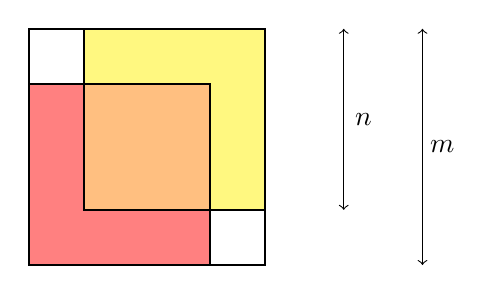
\begin{tikzpicture}
		\draw[thick] (0,0) rectangle (3,3);
		\draw[thick, fill=red!50] (0,0) rectangle (2.3,2.3);
		\draw[thick, fill=yellow!50] (0.7,0.7) rectangle (3, 3);
		\draw[thick, fill=orange!50] (0.7,0.7) rectangle (2.3, 2.3);
		\draw[<->] (4, 0.7)--(4, 3);
		\node at (4.25, 1.85) (n) {$n$};
		\draw[<->] (5, 0)--(5, 3);
		\node at (5.25, 1.5) (m) {$m$};
	\end{tikzpicture}
\end{center}
Amarga $m^2 = 2n^2$, wilayah tumpang tindhih saka rong kothak kang
dawa sisine $n$ nduweni jembar padha karo wilayah kang ora katutupan
dening kothak loro mau; yaiku jembar kothak oranye padha karo gunggung
jembar rong kothak kang ora diwernani. Dadi yen kothak oranye dawa
sisine $p$, lan saben kothak kang ora diwernani dawa sisine $q$, mula
$p^2 = 2q^2$. Nanging saiki $\sqrt{2} = \nicefrac{p}{q}$, kanthi $p < m$
lan $q < n$ sarta $p, q \in \Nat$. Iki kosok balen karo kasunyatan yen
$m$ lan $n$ dipilih sacilik-cilike.

\emph{Kapindho, kanthi formal.} Amarga $m^{2} = 2n^{2}$, mula $m$ iku
genep. (Gampang dituduhake yen $x$ ganjil, mula $x^2$ ganjil.) Dadi
$m = 2r$, kanggo sawatara $r \in \Nat$. Kanthi nata maneh, $2r^2 = n^2$,
		%                \begin{align*}
		%                    (2q)^{2} &= 2n^{2}\\
		%                    4q^{2} &= 2n^{2}\\
		%                    2q^{2} &= n^{2}
		%                \end{align*}
mula $n$ uga genep. Dadi $m$ lan $n$ kalorone genep, mula pecahan
$\nicefrac{m}{n}$ \emph{bisa} disederhanakake maneh. Kosok balen!
\end{proof}

Minangka cathetan sambilan, bukti nganggo diagram iki marakake kita
bisa nyawang maneh bahan saka \olref[his][set][mythology]{sec}.
Tennenbaum (1927--2006) iku matematikawan modern tenan; nanging endahe
bukti iku ora bisa diselaki, ketat babar pisan, lan nggunakake intuisi geometris!

Kepriye wae, wilangan real iku ``luwih jembar'' tinimbang wilangan
rasional. Ing sawenehing teges, ana ``longkangan'' ing wilangan rasional,
lan wilangan real ngisi longkangan mau. Weierstrass mangerteni yen iki
nggambarake siji sipat wilangan real kang mbedakake saka wilangan
rasional, yaiku Sipat Kajangkepan: \emph{Saben himpunan wilangan real kang
ora kosong lan duwe wates ndhuwur mesthi duwe wates ndhuwur paling cilik.}

Gampang dingerteni yen wilangan rasional ora nduweni Sipat Kajangkepan.
Minangka tuladha, gatekna himpunan wilangan rasional kang luwih cilik
tinimbang $\sqrt{2}$, yaiku:
\[
	\Setabs{p \in \Rat}{p^2 < 2 \text{ utawa }p < 0}
\]
Himpunan iki duwe wates ndhuwur ing wilangan rasional; contone, kabeh
!!{element}s luwih cilik tinimbang $3$. Nanging apa wates ndhuwur paling
cilike? Kita kepengin mangsuli ``$\sqrt{2}$''; nanging kita lagi wae weruh
yen $\sqrt{2}$ \emph{dudu} wilangan rasional. Lan ora ana wilangan rasional
\emph{paling cilik} kang luwih gedhe tinimbang $\sqrt{2}$. Dadi himpunan iki duwe
wates ndhuwur nanging ora duwe wates ndhuwur paling cilik. Mula wilangan
rasional ora nduweni Sipat Kajangkepan. Cathetan koreksi sumber OLP-0044:
tandha kurang-saka kang kesasar sawise token unsur ing sumber ora digawa
menyang terjemahan.

Kosok baline, kontinuum ``kudune'' nduweni Sipat Kajangkepan. Kita ora mung
kepengin $\sqrt{2}$ dadi wilangan real; kita kepengin ngisi kabeh
``longkangan'' ing garis rasional. Pancen, kita kepengin kontinuum iku
dhewe ora duwe ``longkangan''. Iki kang bakal dipikolehi liwat Kajangkepan.

\end{document}
